\section{Background}

\subsection{Borealis Airbrakes}
\label{test}
The rocket Borealis (for the 2024 LC competition) was Waterloo Rocketry's first attempt at flying (and for all intents and purposes, developing) active control systems, in the form of airbrakes. At the outset of the airbrakes project, it was envisioned that a working group would develop something like Figure \ref{fig:ab-model}.

\begin{figure}[ht]
    \centering
    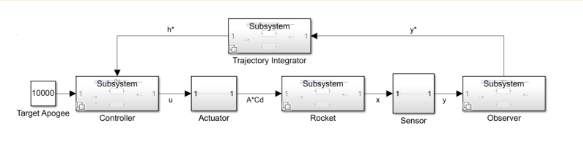
\includegraphics[width=0.8\linewidth]{images-plant/airbrakes.png}
    \caption{Airbrakes control loop structure}
    \label{fig:ab-model}
\end{figure}

Everything except ``Actuator'' and ``Rocket'' were implemented to some degree in the final flight software, but Simulink was never actually used other than to create the above diagram.

A PID controller was ultimately selected for airbrakes because the team lacked the knowledge and scope for anything more complex. This controller was "tuned" using a plugin for OpenRocket (OR) \cite{or-brake}, dynamically modifying the drag force used by OR in its calculations with values produced from external computational fluid dynamics simulations. Later versions included the ability to inject random noise into the state measurements. Under these noisy conditions, simulations suggested the controller could get within about 20m of the target altitude over most of the controllable regime (20,000 +/- 2,000 ft.). 

While much more useful at the time than having no controller-in-loop simulation options at all, the OR plugin was not sustainable. The overlap between Waterloo Rocketry members (and budding control engineers) and Java developers was and still is very small. The final plugin version ran the controller as a binary compiled from the same C source code as the board on the rocket, and while this was also a promising development in the team's testing practices, the process for doing this was even less accessible than running the plugin itself. The plugin project was ultimately an uphill battle to turn OR into something it wasn't meant to be. This motivated the development of a complete simulation alternative in Simulink which could be effectively used for estimator/controller development and validation.
\subsection{Project Jupiter}
Projeto Jupiter is a rocketry team from the University of São Paulo, Brazil. They conveniently already developed most of what is necessary for a plant model of a sounding rocket with canards in Simulink \cite{jupiter-canards}. Rather than trying to start more or less from scratch as it was planned last year, the goal this year was essentially to modify their plant model with our rocket design parameters, verify it for uncontrolled flight against the OR baseline, and then begin simulating the effects of canards.
Although the overall structure of the model was adopted, the actual implemented calculations were either novel or ended up heavily modified. 

\section{Theory}
Compared to a dynamic model of a real launch vehicle, a sounding rocket is considerably simpler. In particular, sloshing, bending, and TVC dynamics do not need to be considered. The rocket can be treated as a single rigid body with time-varying mass and mass distribution. The only forces acting on an uncontrolled rocket are engine thrust, gravity, and drag. Of these, gravity applies no moment by definition, and the moment applied by thrust, due to misalignment with the rocket centre of mass, is constant and typically negligible. Since gravity is well defined and engine thrust is defined empirically via propulsion test data, this leaves the aerodynamic forces and moments as the most complicated aspect of simulation.

The general equation for aerodynamic forces and moments is 
\begin{align}
    F &= \frac{1}{2} \rho V_A^2 C_i(\mathrm{M}, \alpha, \omega) A_r \label{eq:plant-theory-force}
    \\
    M &= F \times d \label{eq:plant-theory-moment}
\end{align}
with the atmospheric density from the standard atmosphere model $\rho$, the local air velocity including wind disturbances $V_A$, and the reference area (e.g. body cross section) $A_r$.
The moment is a cross product of the net force vector $F$ and the vector from the rocket centre of gravity to the centre of pressure $d$.
The coefficient $C_i$ (indexed by the force to be calculated) is an explicit function of the Mach number $\mathrm{M}$, the angle of attack $\alpha$, and the rockets angular velocity $\omega$. 
It depends implicitly on the Reynolds number, on the geometry, surface, and size of the rocket -- in short, the calculation of the coefficients is complicated.

Barrowman \cite{barrowman1967} provides empirical methods for computing the centre of pressure, and the aerodynamic coefficients and derivatives of sounding rockets (for our relevant Mach numbers). 
The method considers the major components (i.e. fins, body nose, etc) of the rocket separately, which simplifies computing and allows easy configuration of parametrized components in implementations (e.g. OpenRocket \cite{niskanen2009, or-manual}).
The characteristic aerodynamic parameters to be calculated are the centres of pressure, normal forcing and picth damping coefficient derivatives, the roll forcing and damping coefficient derivatives, and the drag coefficient \cite{barrowman1967}.
According to Barrowman, the method predicts the aerodynamic characteristics within 10\% of wind tunnel and flight data \cite{barrowman1967}.

The only significant change from an aerodynamics standpoint is the Prandtl factor $\mathcal{B}$, which ``corrects'' the coefficients depending on the Mach number.
Barrowman assumes the Prandtl term to be
\begin{align}
    \mathcal{B}^{-1} &= \frac{1}{\sqrt{\lvert 1-\mathrm{M}^2 \rvert}} \label{eq:plant-theory-prandtl}
\end{align}
which has a singularity at $\mathrm{M} = 1$.
However, the real coefficient does not approach infinity, and both wind tunnel and flight data show that the Prandtl factor peaks at somewhere around 2 or 3 near sonic speeds \cite{stengel2004}.
The implemented correction thus takes $\mathcal{B^{-1}}$ to be the minimum of \ref{eq:plant-theory-prandtl} and 2.

The coefficient of drag ($C_d$) is modelled only as a function of Mach number for a given rocket, using either OR or RASAero data. In the future, other drag models may be considered.

\emph{ToDo: link flight dynamics docs}

\section{Implementation}
The simulation is implemented in Matlab Simulink.
In order to have some semblance of version control (as Simulink \texttt{.slx} files are binary) and to keep the simulation maintainable, the model is in a hierarchical modular architecture.

Each major component of the whole plant, such as flight dynamics, actuators, environmental conditions, or sensor emulation, is encapsulated in its own subsystem. 
The major subsystems are then further structured into layers, e.g. flight dynamics -- forces -- normal forces -- body component lift.
Each layer computes a specific aspect of the physical model,  aggregating contributions from lower-level components. 
This improves traceability, and makes debugging easier by isolating the influence of individual calculations (e.g., lift of fins, body tube, canards).
This modularization eases development and testing of individual components, as intermediate results (e.g. local force contributions) can be verified against theoretical values or simulation baselines. 
The architecture also allows to substitute or refine specific models (e.g. replacing the canard moment calculation with a more detailed version) without disturbing the overall system architecture. 

The model made extensive use of Matlabs' \emph{Aerospace Blockset} (AB), which has ready-to-use implementation blocks for a lot of needed components, e.g. equations of motion, geodetic and magnetic models, IMUs, atmosphere models and accurate wind disturbances, etc.
All units are SI - MKS, to maintain consistency across subsystems and minimize the need for unit conversions. %with the exception of the sensor interface (see below), which uses output units matching the physical IMUs they represent. 

\subsection{Simulation Setup}
The simulation is initialized and parameterized via a configuration script, where the user selects the rocket script to be used.  

A rocket-specific script (e.g. \texttt{borealis.m}) imports a \texttt{.csv} file from an OpenRocket export, containing relevant trajectory and performance data such as time series of thrust, mass, and aerodynamic coefficients.
The OR wind model has not been investigated, and so all OR data is supplied for the no wind case.
Since OpenRocket does not provide complete geometric metadata, this script also explicitly defines additional parameters such as reference dimensions, component locations, mass and moment of inertia.
Another sensor-specific script sets values for sensor parameters such as noise density, bias stability, and limits.
These values are extracted from sensor datasheets or testing.

The configuration script also performs common post-processing on the data as necessary, including numerical differentiation of the time-dependent mass to calculate the mass flow rate, and converting the $C_d$/time and Mach/time series into a direct $C_d$/Mach lookup table. 
This transforms the OR data into the format the simulation expects. 
This modular design allows for rapid integration of new vehicle configurations, provided OpenRocket geometry and performance exports are available.

\subsection{Top Level Plant}
The plant model is composed of three subsystems: the canards actuator, the rocket flight dynamics, and the sensors. Figure \ref{fig:plant-model} shows the connection of these subsystems. 
A visualization subsystem plots the output values of the flight dynamics against the OR results for validation purposes.

\begin{figure}[ht]
    \centering
    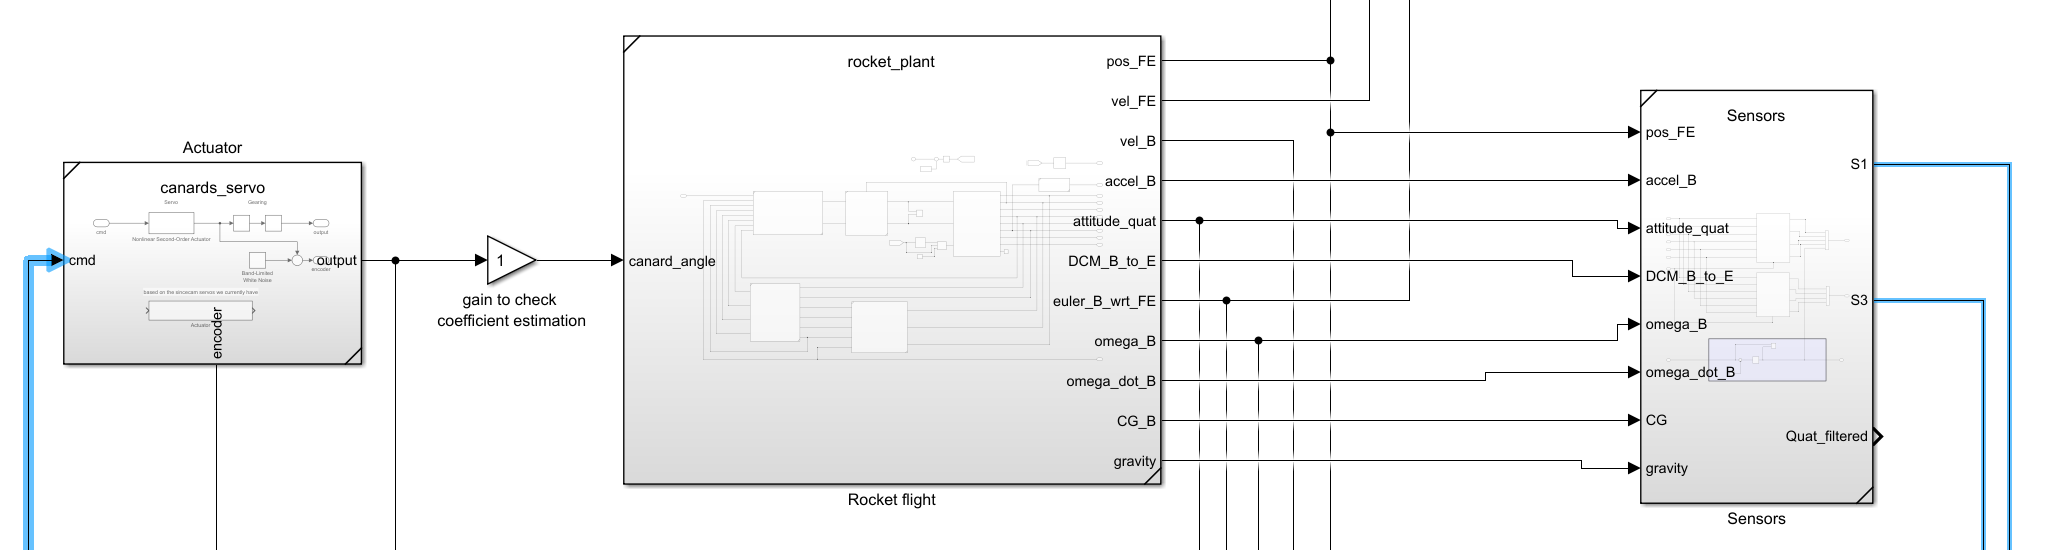
\includegraphics[width=0.9\linewidth]{images-plant/sim_interface.png}
    \caption[Rocket plant model interface]{Rocket plant model interface, with simulated rocket flight (centre), actuator dynamics (left), and sensor models (right).}
    \label{fig:plant-model}
\end{figure}

\subsection{Actuator}
The servo is modelled as a nonlinear second-order system, which includes position and rate limits.
To account for gearing between the servo and the canards, a deadband and hysteresis are used to simulate internal backlash. 
This is in contrast to the linear first-order model used by the estimator.  
To measure the actual canard angle, the actuator is equipped with a rotary potentiometer mounted to one of the canard shafts.
The potentiometer is modelled with additional white noise.
\begin{figure}[ht]
    \centering
    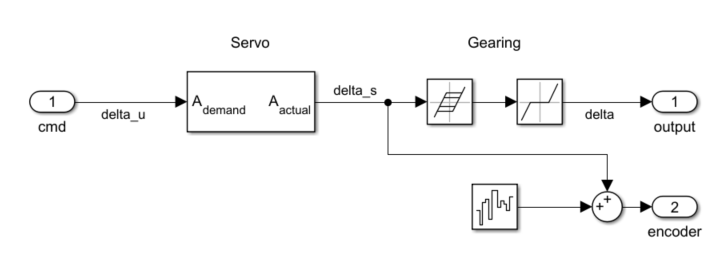
\includegraphics[width=0.5\linewidth]{images-plant/actuator.png}
    \caption{Canards Actuator Dynamics}
    \label{fig:actuator-dynamics}
\end{figure}

\subsection{Sensors}
In order to test the robustness of the controller to real-world sensor outputs, the IMU (accelerometer, gyroscope), magnetometer, and barometer (only pressure) outputs are simulated, adding white noise and other sensor effects (shown in Fig. \ref{fig:imu-subsystem}).
The accelerometer and gyroscope are modelled with AB's IMU block, which accounts for sensor eigendynamics, limits, noise, bias, and (cross-axis) scaling.
The magnetometer uses the International Geomagnetic Reference Field, which is implemented in the AB.
The magnetic field is rotated to the body frame, and noise, scaling, and bias are added to the signal. 
The barometer is modelled with the International Standard Atmosphere block from the AB, and again noise, bias, and scaling is added to the signal.

\begin{figure}[ht]
    \centering
    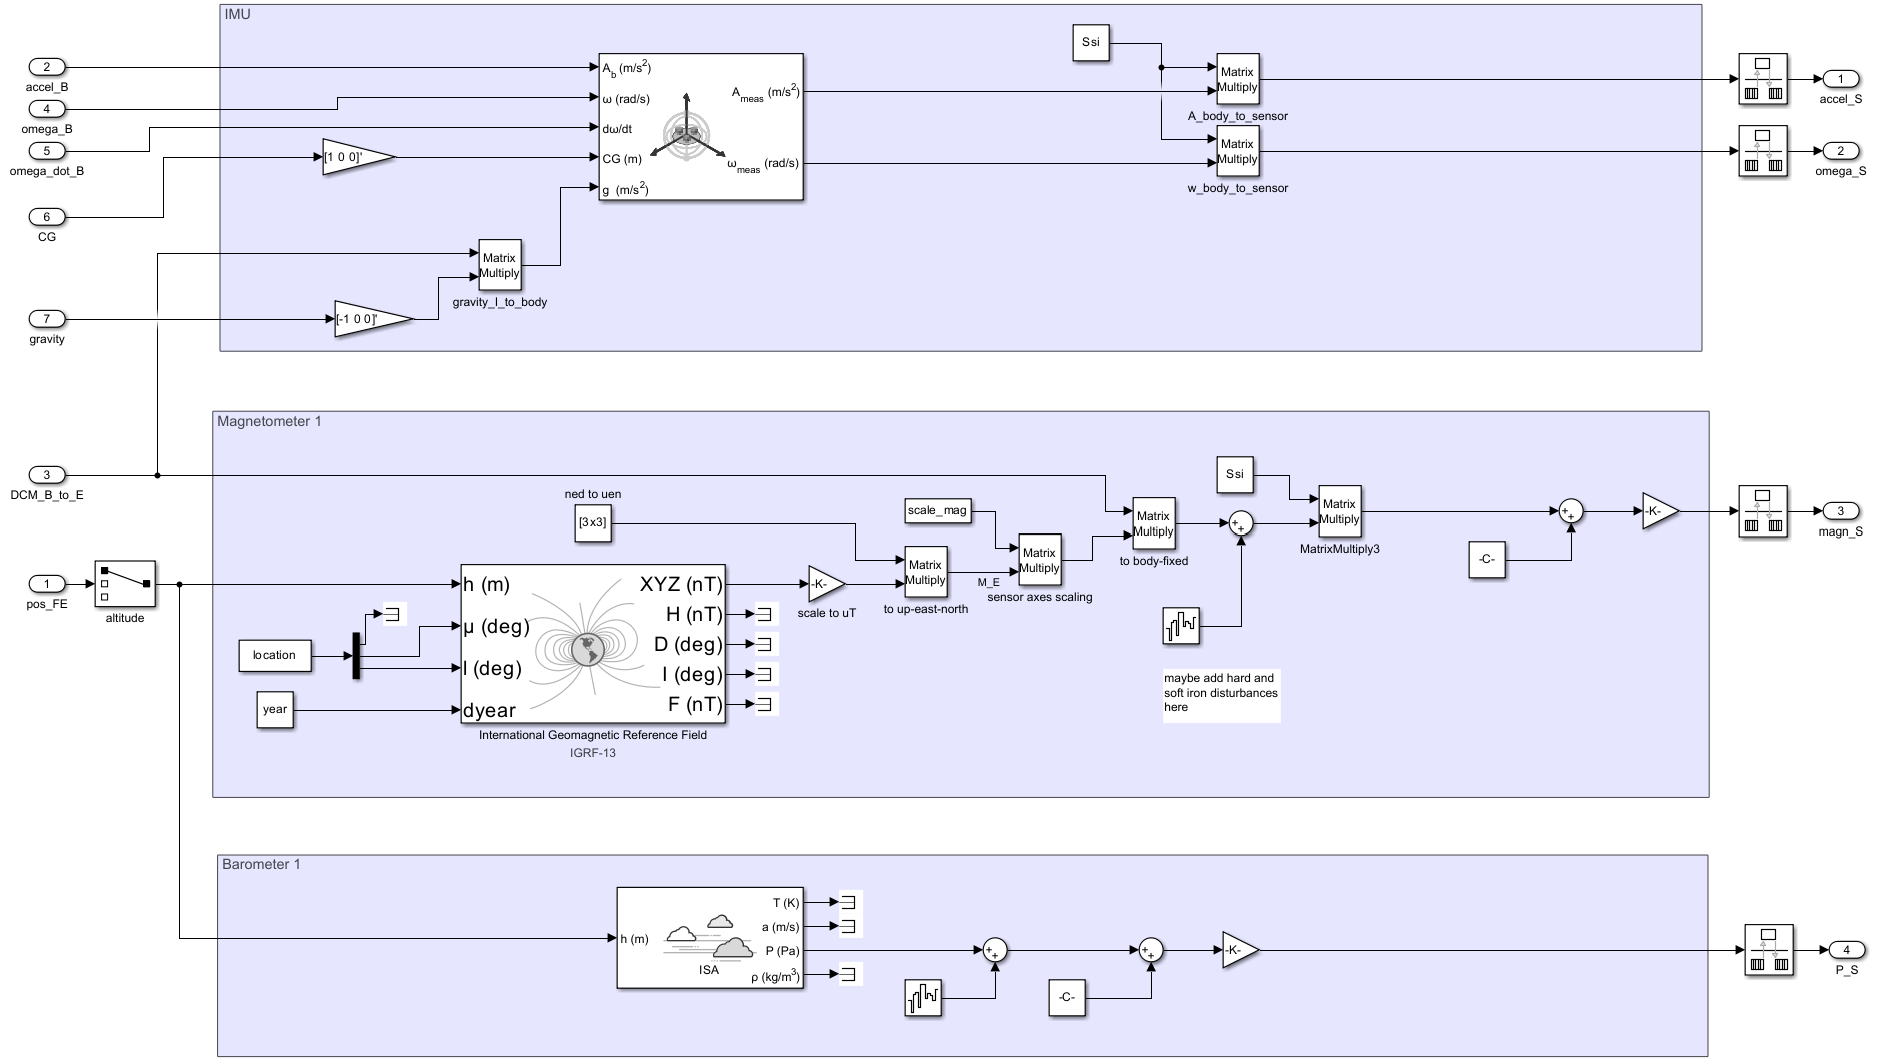
\includegraphics[width=0.7\linewidth]{images-plant/sim_imu.png}
    \caption{Sensor simulation}
    \label{fig:imu-subsystem}
\end{figure}

The sensor simulation is combined to a custom Standard IMU block, which has a mask to input all sensor parameters (shown in Fig. \ref{fig:imu-component}).
The values of those parameters are taken from datasheet values, and may be adjusted based upon sensor testing.
The estimator is connected to 3 unlike IMUs for redundancy, and to alleviate saturation. The Movella MTi-630 is an integrated Altitude and Heading Reference System (AHRS), which contains its own onboard orientation filter. 
The LSM6DSV32X and AltIMU-10 are an IMU and IMU carrier board respectively. They are henceforth all referred to as ``IMUs''. In the final implementation, data is sampled from all IMUs at the nominal execution rate, concatenated, and passed to the estimator for processing.

\begin{figure}[ht]
    \centering
    \begin{subfigure}{0.45\textwidth}
        \centering
        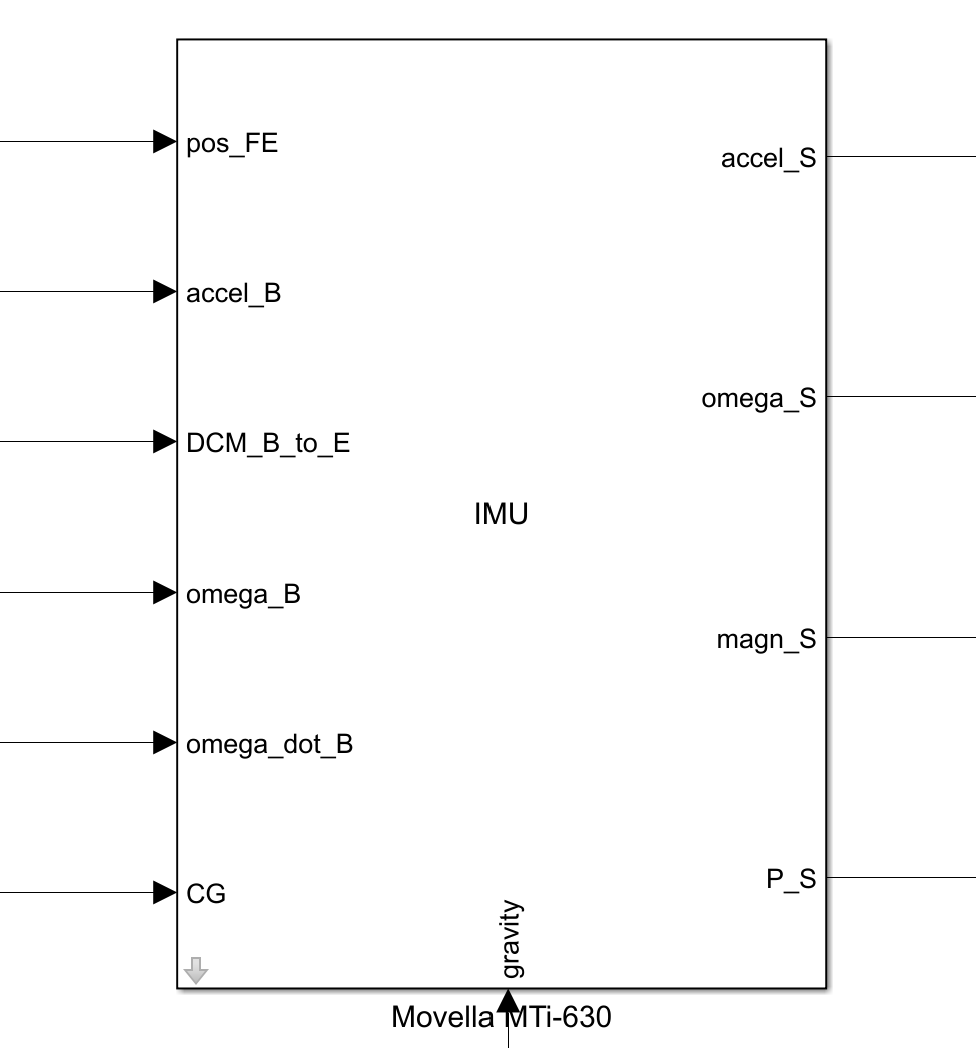
\includegraphics[width=0.5\linewidth]{images-plant/sim_imu_instance.png}
        \caption{Standard IMU component block}
        \label{fig:imu-component_inst}
    \end{subfigure}
    \begin{subfigure}{0.45\textwidth}
        \centering
        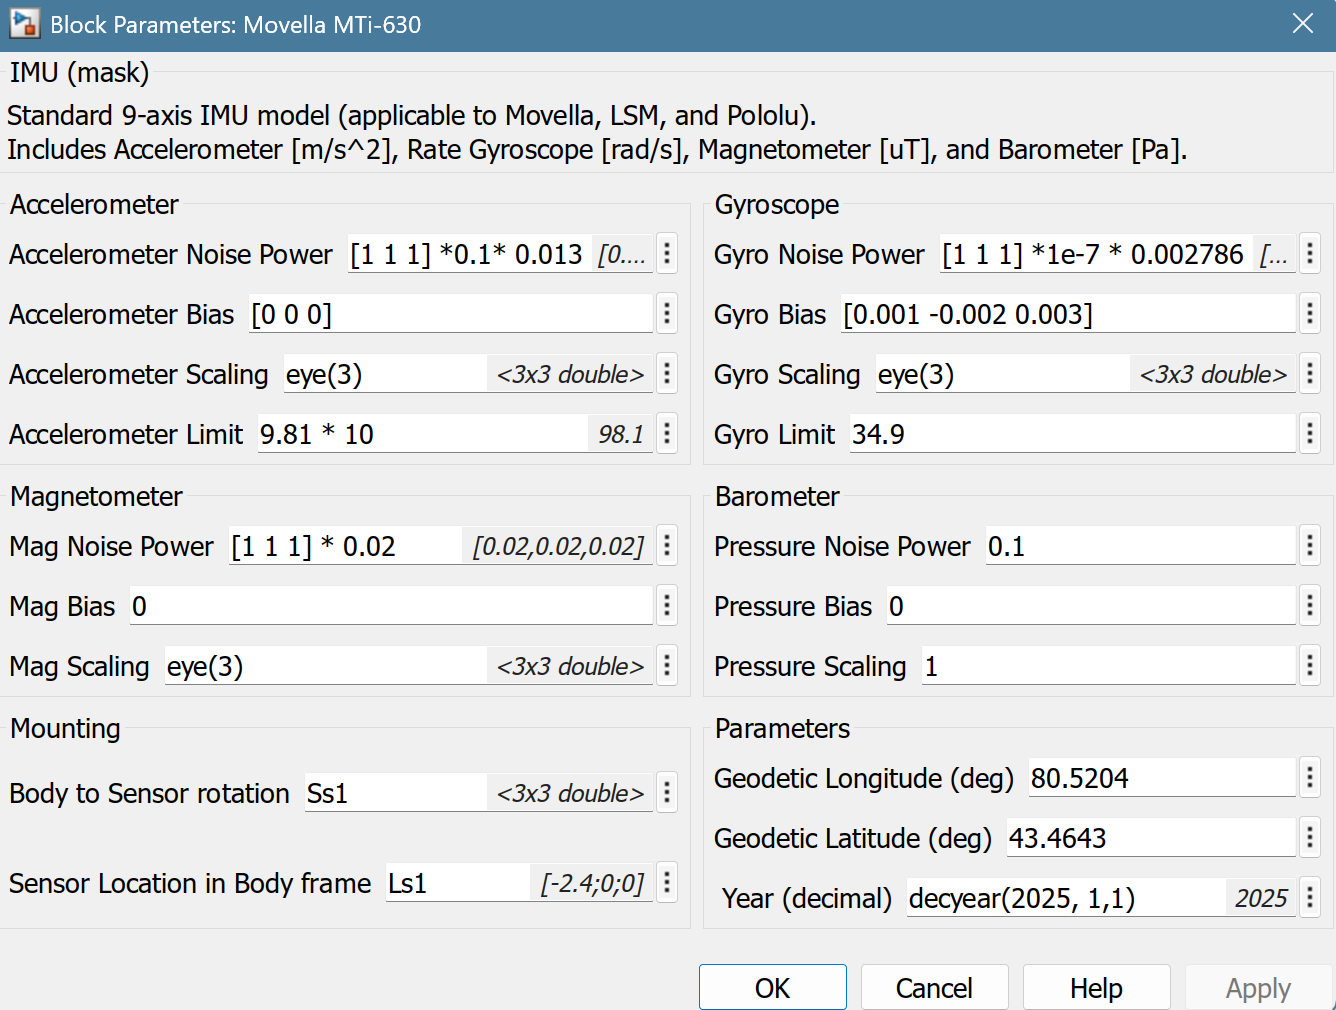
\includegraphics[width=0.8\linewidth]{images-plant/sim_imu_mask.png}
        \caption{IMU instance parameter interface}
        \label{fig:imu-component_mask}
    \end{subfigure}
    \caption{Standard IMU component instance}
    \label{fig:imu-component}
\end{figure}

\subsection{Rocket Flight}
All time-based look-up tables (e.g. thrust, mass, centre of gravity) with OR data are connected to a global clock.
To simulate idle time on the launch rail, a user-defined idle duration can be specified via the initialization script. This  offsets the simulation time prior to OpenRocket’s nominal $t=0$, effectively holding the rocket in a static state (with rail constraints) before powered ascent begins. 
This is a necessity for accurately modelling the pre-launch controller initialization.

\subsubsection{6DOF Variant Mass Model}
The core of the rocket flight dynamics model is the ``Simple Variable Mass 6DOF'' block by the Aerospace Blockset, providing equations of motion in six degrees of freedom.
It takes in net force and moment vectors about the rocket centre of mass, and outputs the kinematic states of position, velocity, acceleration, orientation, angular velocity and acceleration.
Note that the inputs are provided in the body fixed frame, with the X-axis coincident with the longitudinal axis of the rocket body. The translational position and velocity are provided in the flat earth reference frame. The origin of this inertial frame is arbitrary for dynamics purposes, but is effectively the position of the launch rail on the earth surface.
The 6DOF block does not output mass vs time, instead providing inputs for starting mass, ending mass, and mass flow rate $\frac{dm}{dt}$. 
The moment of inertia is interpolated linearly between initial and final moments of inertia, using the mass flow rate $\frac{dm}{dt}$.

\begin{figure}[ht]
    \centering
    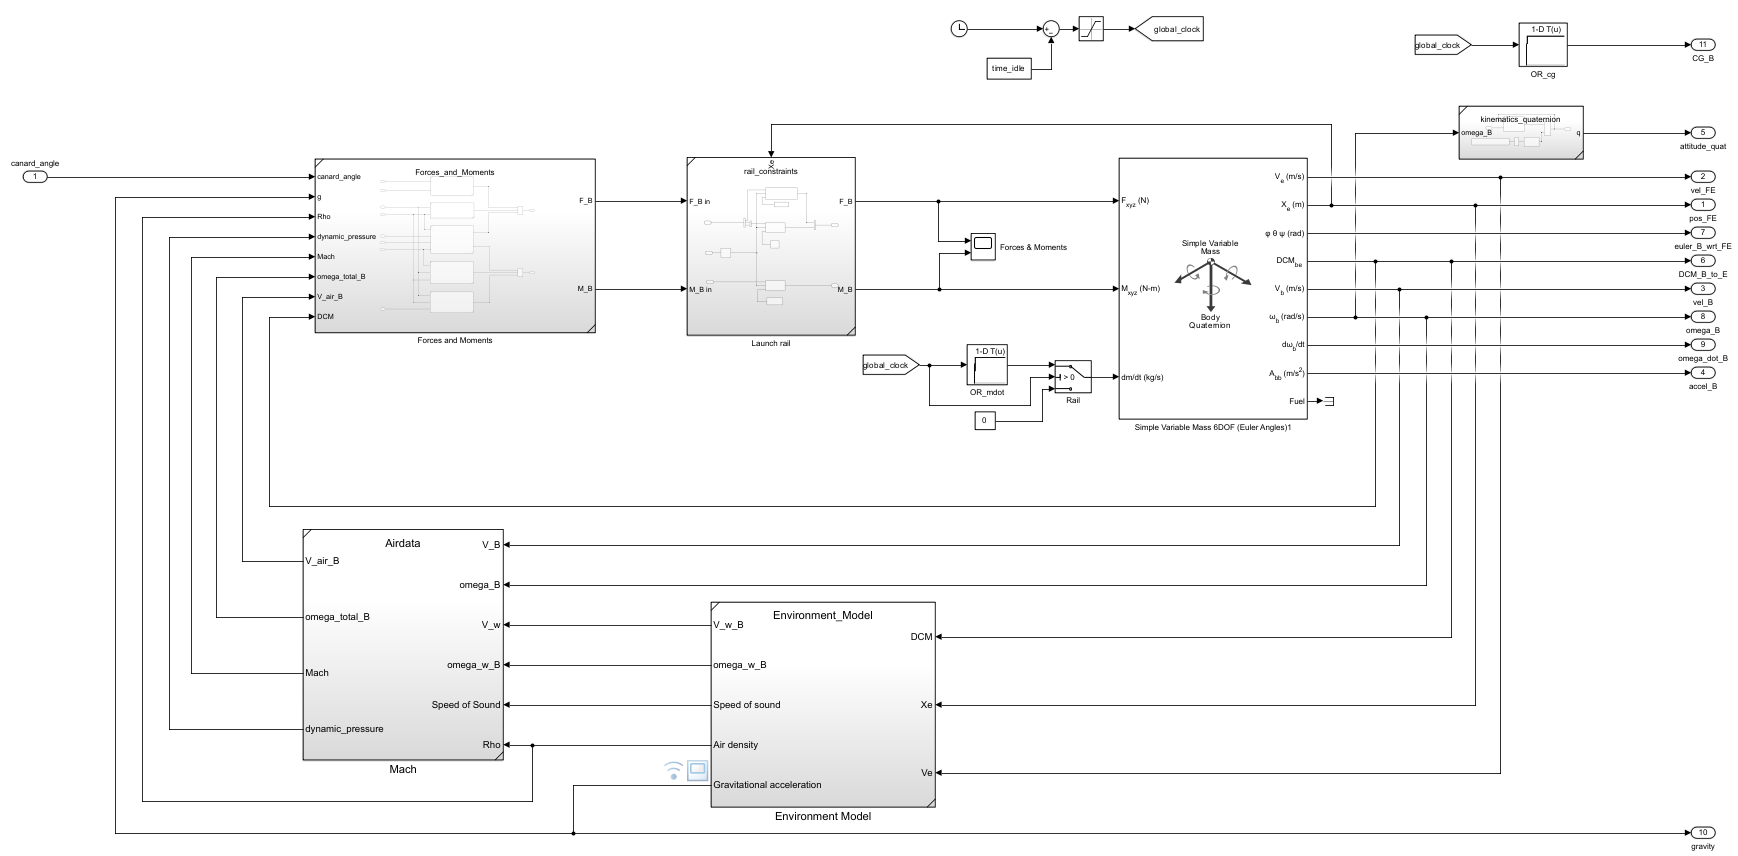
\includegraphics[width=0.9\linewidth]{images-plant/sim_rocket.png}
    \caption[Rocket flight system]{Rocket flight system, with 6DOF Equations of Motion, wind disturbances, external forces and moments, rail constraints.}
    \label{fig:rocket-flight}
\end{figure}


\subsubsection{Environment, Air data}
To accurately model gravitation and the surrounding air, environment blocks from the AB are used.
%Due to compatibility and internal dependencies within the AB, 
The WGS84 Earth model is used where applicable for geodetic reference, such as coordinate transformations and gravitational acceleration.
The air is modelled using the International Standard Atmosphere, which computes air density and the local speed of sound according to the current altitude.

The Airdata subsystem calculates the rocket velocity relative to the oncoming air $V_A$, adding the velocity relative to the Earth and the local wind velocity vector.
Using the environment data, the Mach number and dynamic pressure ($0.5 \rho V_A^2$) are calculated.


\subsubsection{Wind disturbances}
The wind environment is modelled as a layered system combining steady-state wind, stochastic turbulence, and discrete gust events. 
The steady-state wind and stochastic turbulence operate similar to OpenRocket \cite{niskanen2009}. 
The baseline wind assumes a constant wind velocity over all altitudes. 
While this assumption simplifies the vertical wind profile, it remains sufficient in the absence of detailed meteorological data.
Superimposed on the steady wind is a stochastic turbulence using  pink noise (with higher noise amplitude at lower frequencies, 1/f) 
This introduces realistic low-frequency variability to the wind vector, creating stochastic lateral and vertical disturbances. This stochastic turbulence is also responsible for all rotational components of the wind pertubations. 

Additionally, discrete gusting is added to the baseline and stochastic winds, which allows the user to define transient changes in wind velocity.
Each gust is specified by magnitude, direction, time of onset and duration.

\subsubsection{Rail constraints}
While the rocket remains on the launch rail, its motion is constrained to a single degree of freedom in the rocket forward direction. 
This models the effect of launch lug constraints, which restrict lateral and angular motion prior to rail clearance to keep the rocket vertical (until a sufficient vertical velocity is achieved, to prevent wind-induced pitch over).

This is implemented by filtering out all forces and moment but the positive forces in the x-direction, while the rocket is under a certain altitude -- in this case the start altitude, plus the length of the launch rail.
This effectively locks the vehicle in place until liftoff and prevents any unrealistic drift or rotation while idle on the rail. It also ensures that simulation of rail clearance behavior and initial angular acceleration are accurate.

\subsection{Forces and Moments}
The total force and moment vectors acting on the rocket are computed by summing contributions from gravity, propulsion, and aerodynamics, as shown in Fig. \ref{fig:sim-forces}.
These forces and moments are computed in the rocket’s body-fixed coordinate frame, relative to the instantaneous centre of gravity.

\begin{figure}[ht]
    \centering
    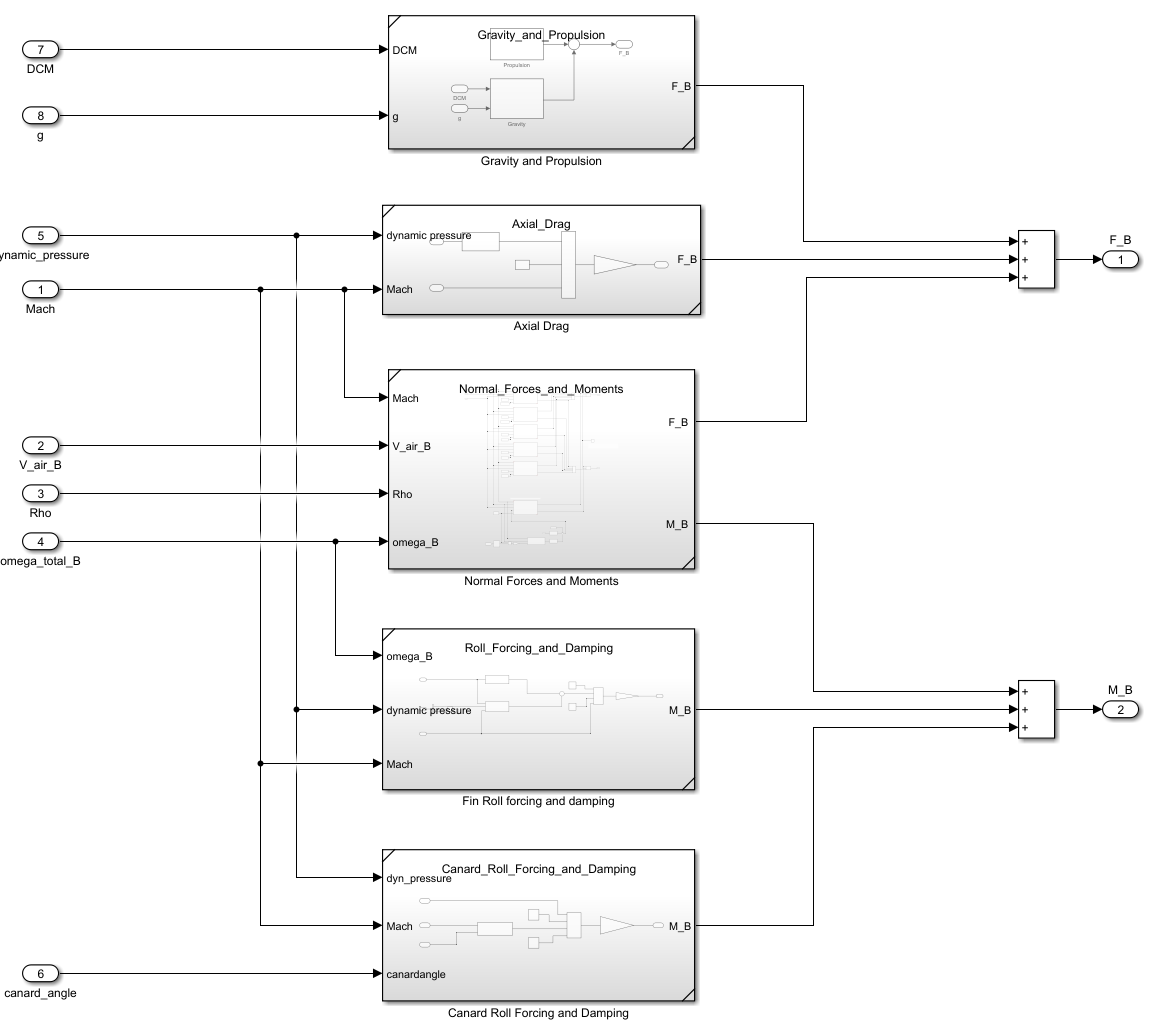
\includegraphics[width=0.5\linewidth]{images-plant/sim_forces.png}
    \caption{External forces and moments}
    \label{fig:sim-forces}
\end{figure}

\subsubsection{Propulsion}
The propulsion force is modelled using a time-series look-up table, indexed by the global clock. 
This thrust curve provides instantaneous thrust at discrete time points.
It is imported from a preprocessed OR export (or directly from static fire test data).

The thrust vector is assumed to align with the rocket longitudinal axis (body-x), and thus produces no moment about the rocket centre of gravity.
Gimballing or off-axis thrust components are currently not modelled, but could be added later on. 

\subsubsection{Aerodynamic Drag force}

Aerodynamic drag is implemented via a $C_d$/Mach look-up table, generated from OR data. 
This table provides the drag coefficient $C_d$ as a function of Mach number, based on vehicle geometry defined in OR.

The drag force is computed with this $C_s$ and the dynamic pressure, as it is assumed the vector of oncoming air is mostly in the x-direction. 
The drag is 
\begin{equation}
    F_D = 0.5 \rho V_{A}^2 \, C_d A_{r}
\end{equation}
with the atmospheric density $\rho$, the local air velocity $V_A$, and the body cross section $A_r$.

 Corrections for angle of attack and transonic behavior are not yet implemented in this module but may be included later. 

\subsubsection{Aerodynamic Roll torque} 
The roll dynamics of the rocket are driven primarily by the aerodynamic forces generated by the fins and canards.
For flexibility they are split into separate components and treated independently. This allows the canards to be handled with more detail or with different aerodynamic models if needed, and to easier accommodate different flight regimes or experimental configurations.

In the contribution of the fins, the aerodynamic coefficients and variable derivatives are computed in pre-processing using Barrowman's equations \cite{barrowman1967}, and then fed into the Simulink model. 
The Barrowman method takes into account the fin's aerodynamic area, span, mean chord, and the angle of attack to compute the moment coefficients.
The derivatives are used by the ``roll forcing and damping block'' in the plant model, the forcing component is shown in Fig. \ref{fig:roll-torque}. 

\begin{figure}[ht]
    \centering
    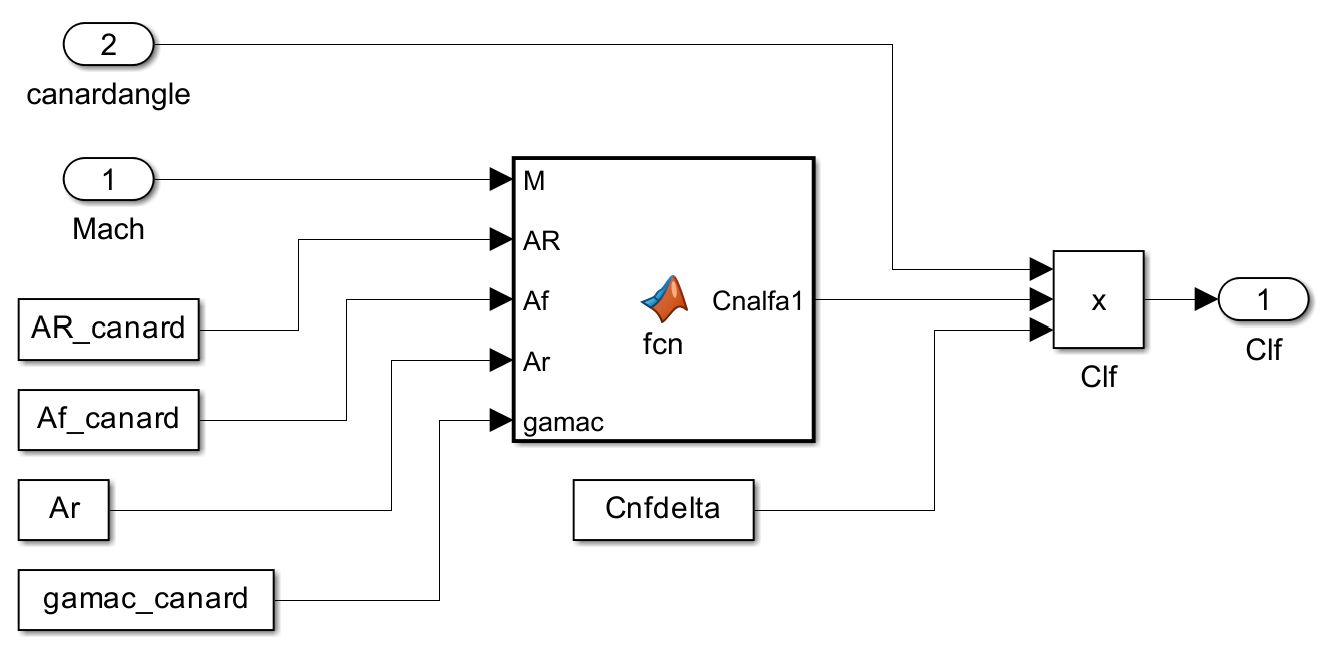
\includegraphics[width=0.4\linewidth]{images-plant/sim_roll_forcing.png}
    \caption{Canard roll torque, roll forcing component}
    \label{fig:roll-torque}
\end{figure}

While the fins are treated using Barrowman's equations, the canard contribution to roll dynamics are handled slightly differently to correspond to aerodynamic development done by the Flight Dynamics subsystem \cite{team-flight-luca}.
The coefficient of the canards is computed using thin airfoil theory for low aspect delta wings with supersonic leading edges, found in Stengel \cite[p. 73]{stengel2004}.


\subsubsection{Aerodynamic Normal forces and Moments}
The methodology used to compute the normal force components, which affect pitch dynamics of the rocket, is the same as that of OpenRocket \cite[sec. 3.2.1]{or-manual}. The rocket body is divided into its major components: nosecone, body, fin, tail, and canards.
Each component is treated as a separate aerodynamic entity, and the normal force and moment contributions from each are computed individually based on local airflow conditions.
The local velocity of oncoming air at the component centre of pressure is computed to calculate the normal force and moment vectors, along with the normal force coefficient derivative $C_{N_\alpha}$.
Each component's contribution to the normal force vector is given by:
\begin{align}
    F_{N} &= 0.5 \rho V_A^2 C_{N_\alpha} \alpha A_r 
    & 
    M_{N} &= F_{N} \times d
\end{align}

This functionality is encapsulated in a generic "lift component" block, whose internals are shown in Fig. \ref{fig:lift-component}.
The individual component forces and moment vectors are added to produce a net aerodynamic normal force and pitch moment.
%, as shown in Fig. \ref{fig:normal-force}.

This approach is integral to predicting the passive aerodynamic stability of the rocket, the rocket is passively stable if the the net moment produced by any angle of attack is driving the angle of attack to zero -- i.e. the rocket is stable if it turns into the wind.

\begin{figure}[ht]
    \centering
    \begin{subfigure}{0.45\textwidth}
        \centering
        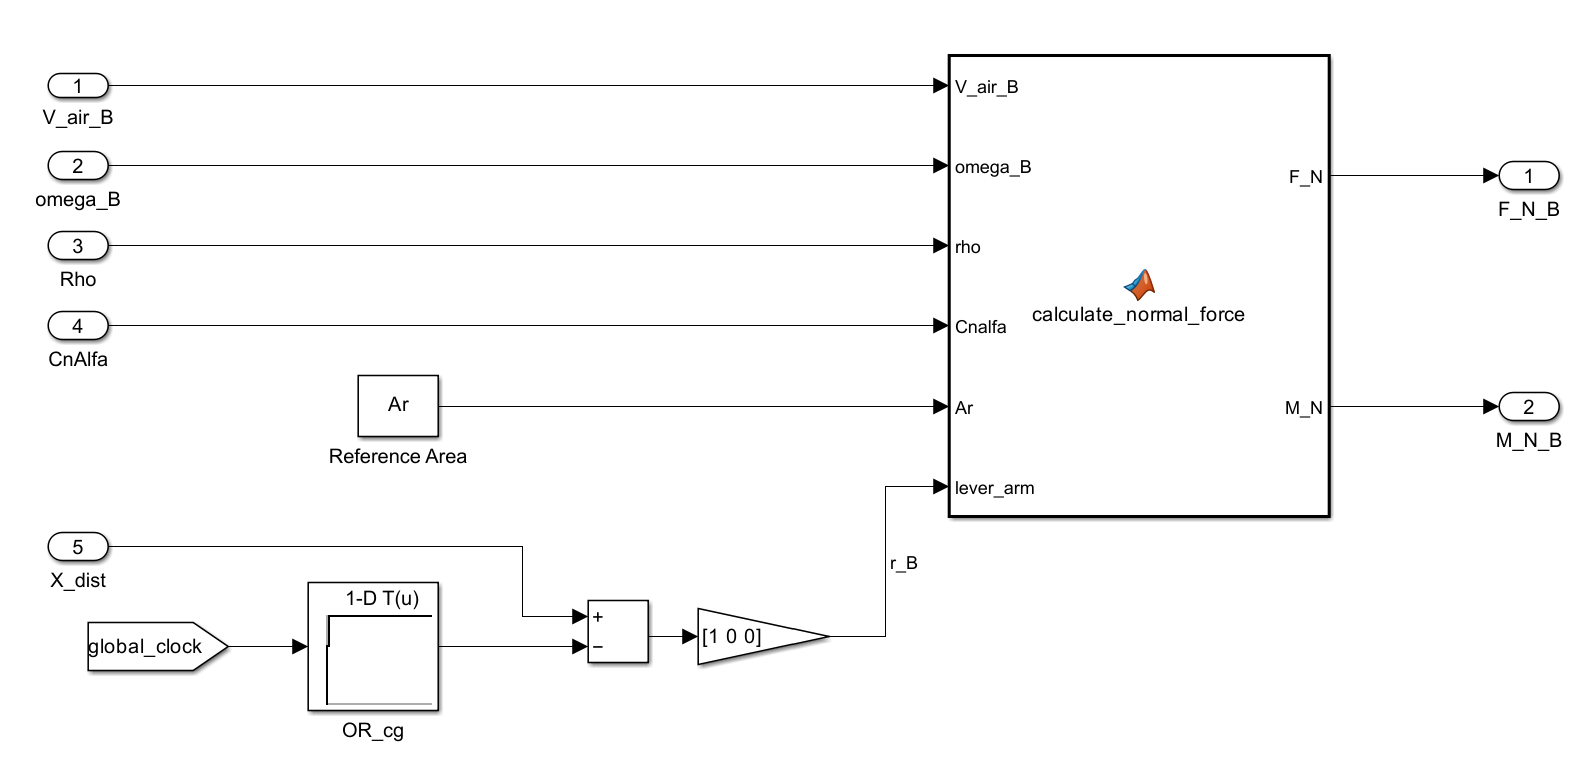
\includegraphics[width=0.9\linewidth]{images-plant/sim_lift_block.png}
        \caption{Lift component block structure}
        \label{fig:lift-component-block}
    \end{subfigure}
    \begin{subfigure}{0.54\textwidth}
        \centering
        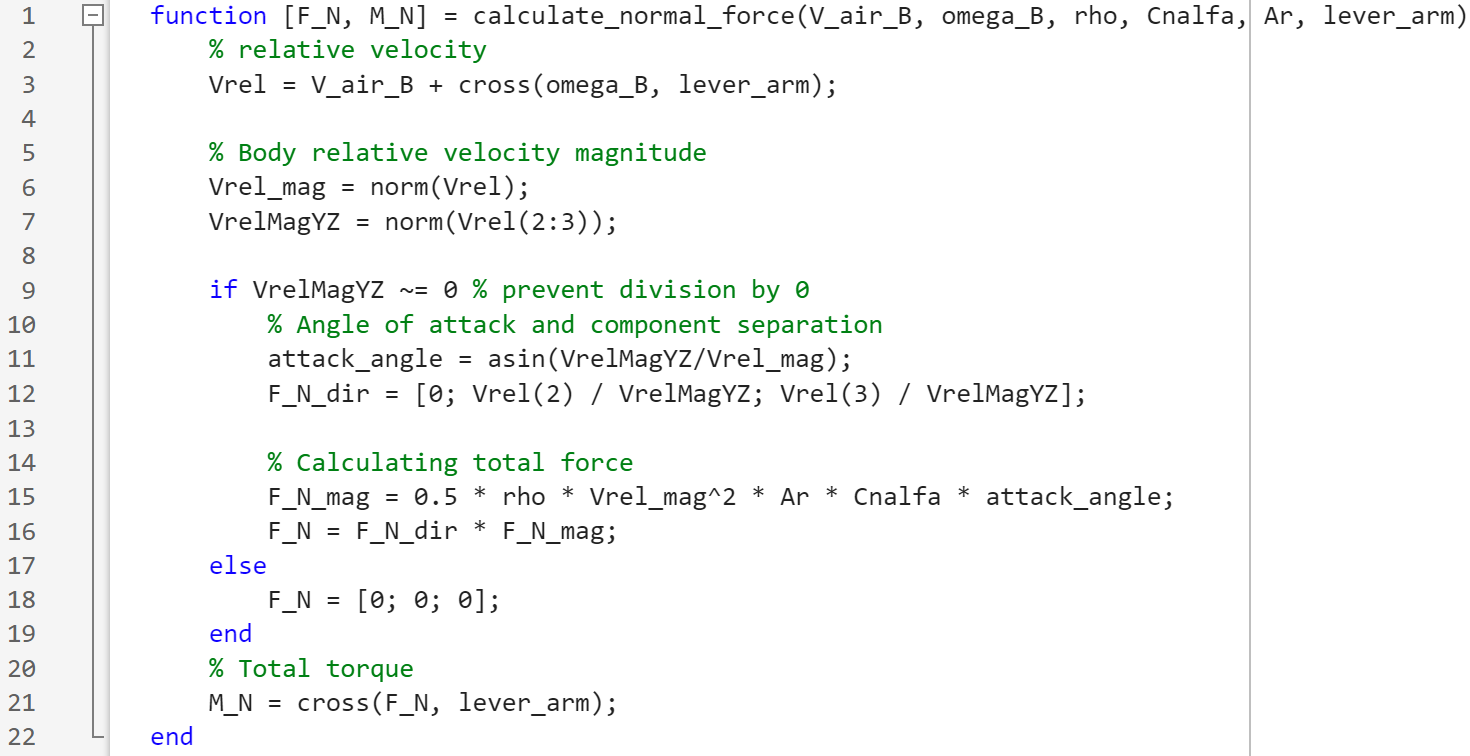
\includegraphics[width=0.9\linewidth]{images-plant/sim_lift_equation.png}
        \caption{Lift component calculation}
        \label{fig:lift-component-eq}
    \end{subfigure}
    \caption{Lift component subsystem}
    \label{fig:lift-component}
\end{figure}

%\begin{figure}[ht]
%    \centering
%    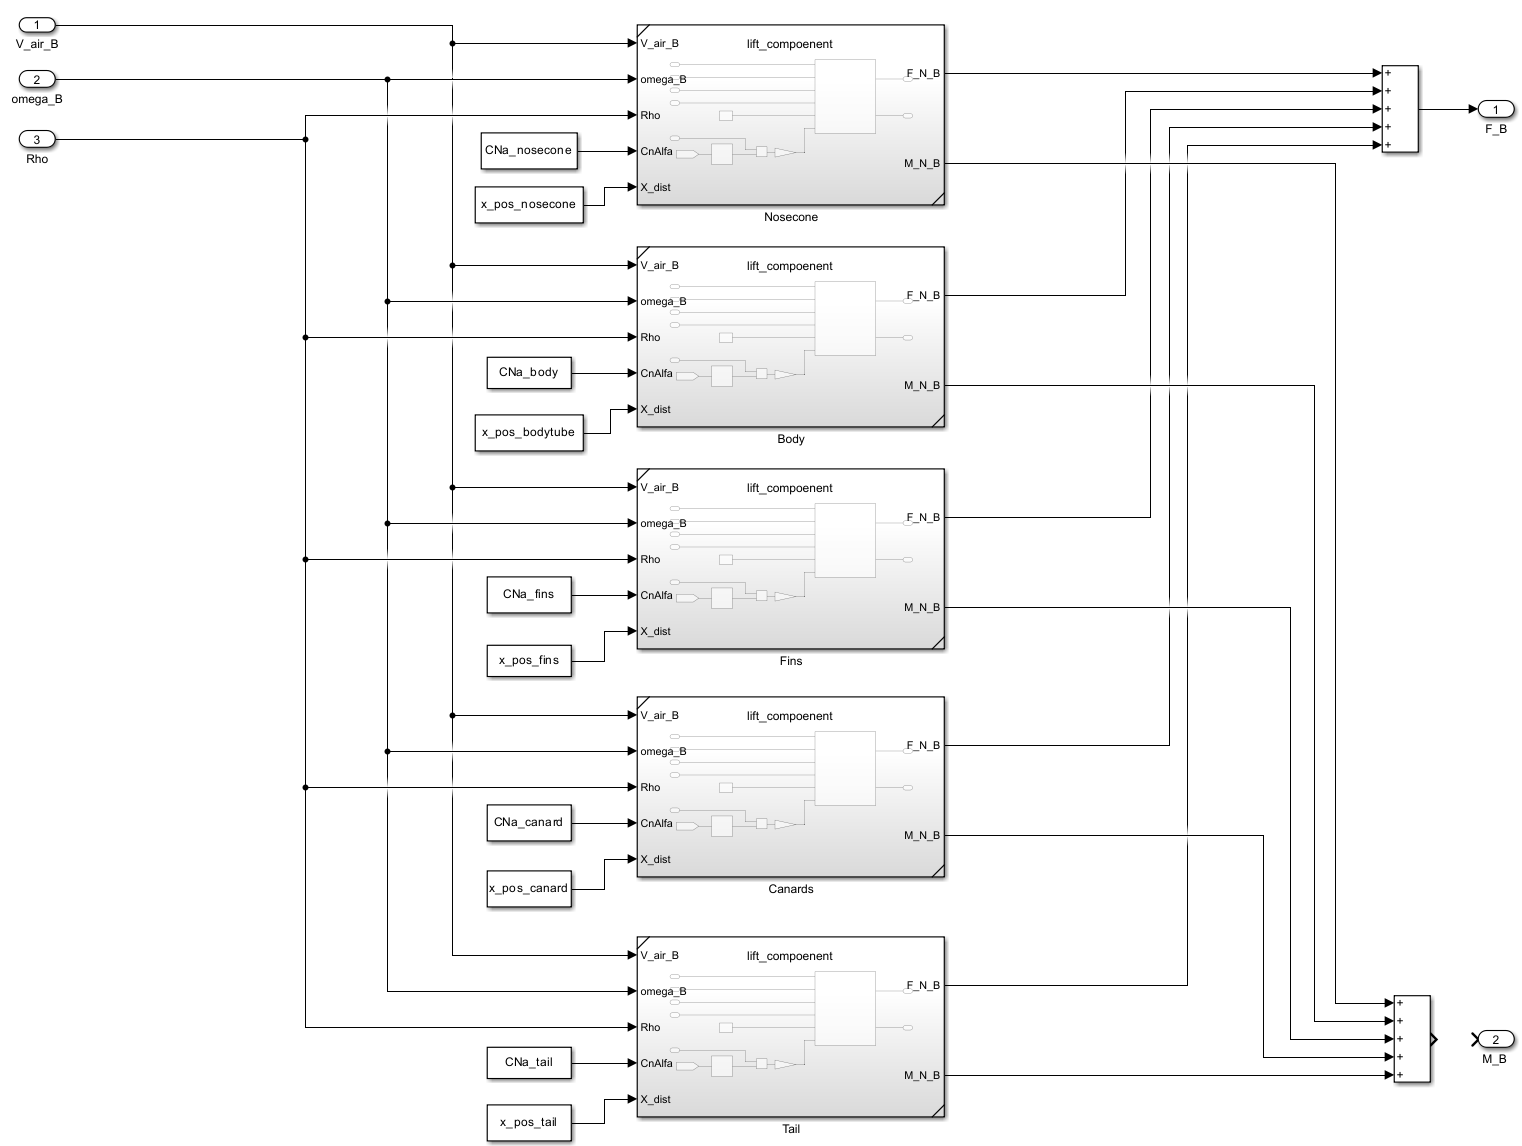
\includegraphics[width=0.65\linewidth]{images-plant/sim_forces_normal.png}
%    \caption{Normal Force and Moment}
%    \label{fig:normal-force}
%\end{figure}
